\documentclass[12pt]{article}

\usepackage[T1]{fontenc}
\usepackage[utf8]{inputenc}
\usepackage[english]{babel}
\usepackage{geometry}
\usepackage{graphicx}
\usepackage{booktabs}
\usepackage{array}
\usepackage{longtable}
\usepackage{float}
\usepackage{amsmath, amssymb}
\usepackage{caption}
\usepackage{xcolor}
\usepackage{hyperref}
\usepackage{setspace}
\usepackage{titling}

\geometry{margin=1in}
\setlength{\parskip}{0.7em}
\setlength{\parindent}{0pt}
\hypersetup{colorlinks=true, linkcolor=black, urlcolor=blue, citecolor=black}

\definecolor{usdred}{RGB}{161,7,43}

\pretitle{\begin{center}\LARGE\bfseries}
\posttitle{\par\end{center}}
\preauthor{\begin{center}\large}
\postauthor{\par\end{center}}
\predate{\begin{center}\normalsize}
\postdate{\par\end{center}}

\title{Room Occupancy Detection Using Environmental Sensor Data}
\author{Benjamin van Rhee\\Department of Computer Science\\University of South Dakota\\CSC 444}
\date{Spring 2026}

\begin{document}

\begin{titlepage}
    \centering
    {\color{usdred}\rule{\textwidth}{1.2pt}\par}
    \vspace{1.2cm}
    {\Huge\bfseries Room Occupancy Detection Using Environmental Sensor Data\par}
    \vspace{1.2cm}
    {\Large Benjamin van Rhee\par}
    \vspace{0.4cm}
    {\large Department of Computer Science\par}
    {\large University of South Dakota\par}
    {\large CSC 444\par}
    \vfill
    {\large Final Report\par}
    \vspace{0.3cm}
    {\large Spring 2026\par}
    \vspace{1.2cm}
    {\color{usdred}\rule{\textwidth}{1.2pt}\par}
\end{titlepage}

\begin{abstract}
This project studies room occupancy detection as a binary classification problem using environmental sensor data. The dataset comes from the UCI Machine Learning Repository and contains 20,560 observations with measurements for Temperature, Humidity, Light, CO$_2$, and HumidityRatio, along with a binary occupancy label. Two supervised learning methods were compared: Logistic Regression and Random Forest. The goal was to test whether a simple linear model could perform competitively against a more complex ensemble method for occupancy detection. Results showed that Logistic Regression with feature scaling produced the best overall performance, reaching an F1 score of 0.9694 on the validation split and 0.9824 on the final holdout test split. Random Forest also performed well, but it was slightly weaker overall. Feature importance analysis showed that Light and CO$_2$ were the strongest predictors of occupancy. These findings suggest that occupancy can be detected accurately using common building sensor data without relying on invasive sensing methods such as cameras.
\end{abstract}

\section{Introduction}
Occupancy detection is an important problem in smart buildings and Internet of Things systems. Reliable occupancy estimates can improve heating, cooling, lighting, and ventilation control, which can reduce energy use and improve occupant comfort. In practice, building systems often rely on environmental sensor measurements instead of cameras because those sensors are less invasive and easier to deploy.

This project uses the UCI Occupancy Detection dataset to predict whether a room is occupied. The problem is a supervised binary classification task where the target label is \texttt{Occupancy}, and the input features are environmental sensor readings. The dataset is suitable for a class project because it is clean, has no missing values, and has already been used in published research on occupancy detection.

The main objective of this project is to compare a simple model and a more complex model on the same dataset. Logistic Regression was selected as the baseline because it is fast, interpretable, and commonly used for binary classification. Random Forest was selected because it can capture more complex nonlinear relationships between features. The main research question is whether the added complexity of Random Forest leads to better performance than Logistic Regression on this occupancy task.

\section{Dataset}
The project uses the three occupancy files included in the provided dataset folder: \texttt{datatraining.txt}, \texttt{datatest.txt}, and \texttt{datatest2.txt}. The files were used as predefined dataset splits rather than creating new random splits.

\begin{table}[H]
\centering
\caption{Dataset Splits}
\begin{tabular}{lc}
\toprule
Split & Rows \\
\midrule
Training & 8,143 \\
Validation & 2,665 \\
Final holdout test & 9,752 \\
\bottomrule
\end{tabular}
\end{table}

Each record contains the following fields: Temperature, Humidity, Light, CO$_2$, HumidityRatio, and Occupancy. The \texttt{date} column was parsed as a timestamp but was not used directly as a predictive feature in the main experiments. This kept the comparison focused on the environmental sensor values listed in the proposal.

\subsection{Class Balance}
The dataset is moderately imbalanced toward the not occupied class, which means accuracy alone is not enough to evaluate performance.

\begin{table}[H]
\centering
\caption{Class Balance Across Splits}
\begin{tabular}{lrr}
\toprule
Split & Not Occupied & Occupied \\
\midrule
Training & 6,414 & 1,729 \\
Validation & 1,693 & 972 \\
Test & 7,703 & 2,049 \\
\bottomrule
\end{tabular}
\end{table}

\begin{figure}[H]
    \centering
    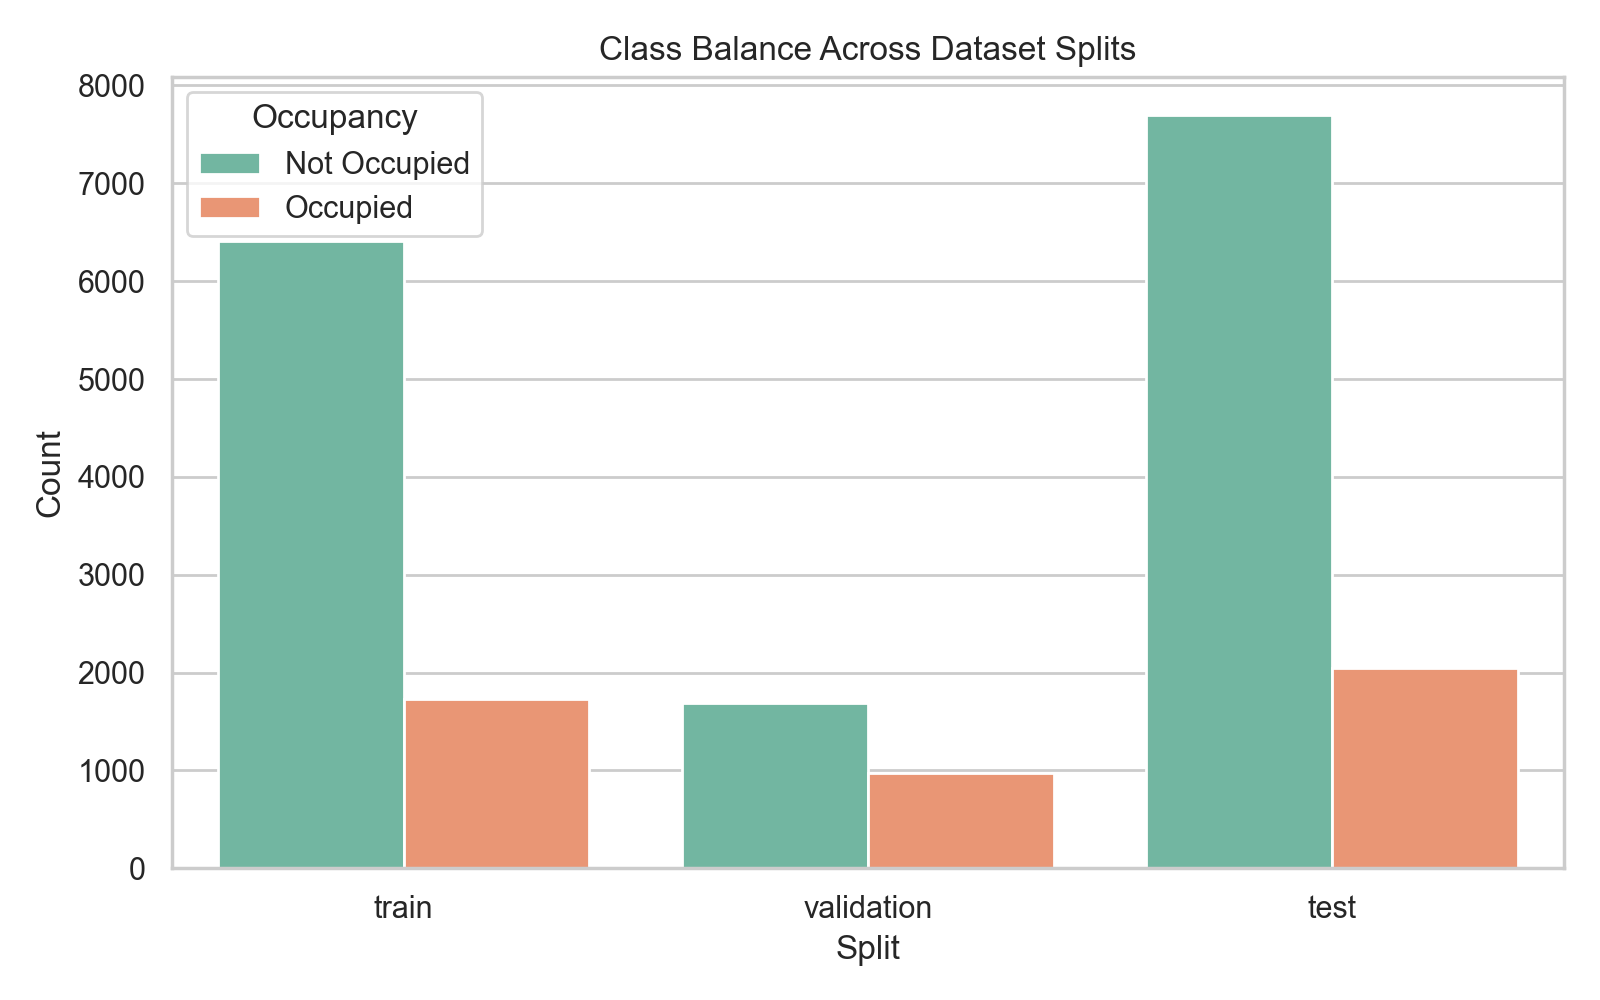
\includegraphics[width=0.9\textwidth]{figures/class_balance.png}
    \caption{Class balance across training, validation, and test splits.}
\end{figure}

\section{Methodology}
\subsection{Preprocessing}
The dataset required very little cleaning. The first column in each file is a row index and was ignored when loading the data. The remaining fields were read with the \texttt{date} column parsed as a timestamp. No missing values were found, so imputation was not required.

The final feature set used for modeling was Temperature, Humidity, Light, CO$_2$, and HumidityRatio. The target variable was the binary \texttt{Occupancy} label.

\subsection{Models}
Three model variants were evaluated during the comparison stage:
\begin{enumerate}
    \item Logistic Regression without feature scaling
    \item Logistic Regression with standardization
    \item Random Forest
\end{enumerate}

The scaled Logistic Regression model used a \texttt{StandardScaler} inside a scikit learn pipeline to avoid leakage. Random Forest was trained with 300 trees and a fixed random seed for reproducibility.

\subsection{Evaluation Metrics}
The models were compared using accuracy, precision, recall, F1 score, and confusion matrices. The validation split was used for model comparison. After selecting the best approach, the top models were retrained on the combined training and validation data and then evaluated once on the final holdout test split.

\section{Exploratory Data Analysis}
Summary statistics from the training split showed that the feature scales are quite different. For example, Light ranges from 0 to 1546.333, while HumidityRatio remains near 0.004 on average. This difference in scale is one reason feature standardization was tested for Logistic Regression.

The feature correlation heatmap suggests that Light has the strongest direct association with occupancy, with CO$_2$ also showing a meaningful relationship. This pattern matches the intuition that occupied spaces typically have more lighting activity and human generated CO$_2$.

\begin{figure}[H]
    \centering
    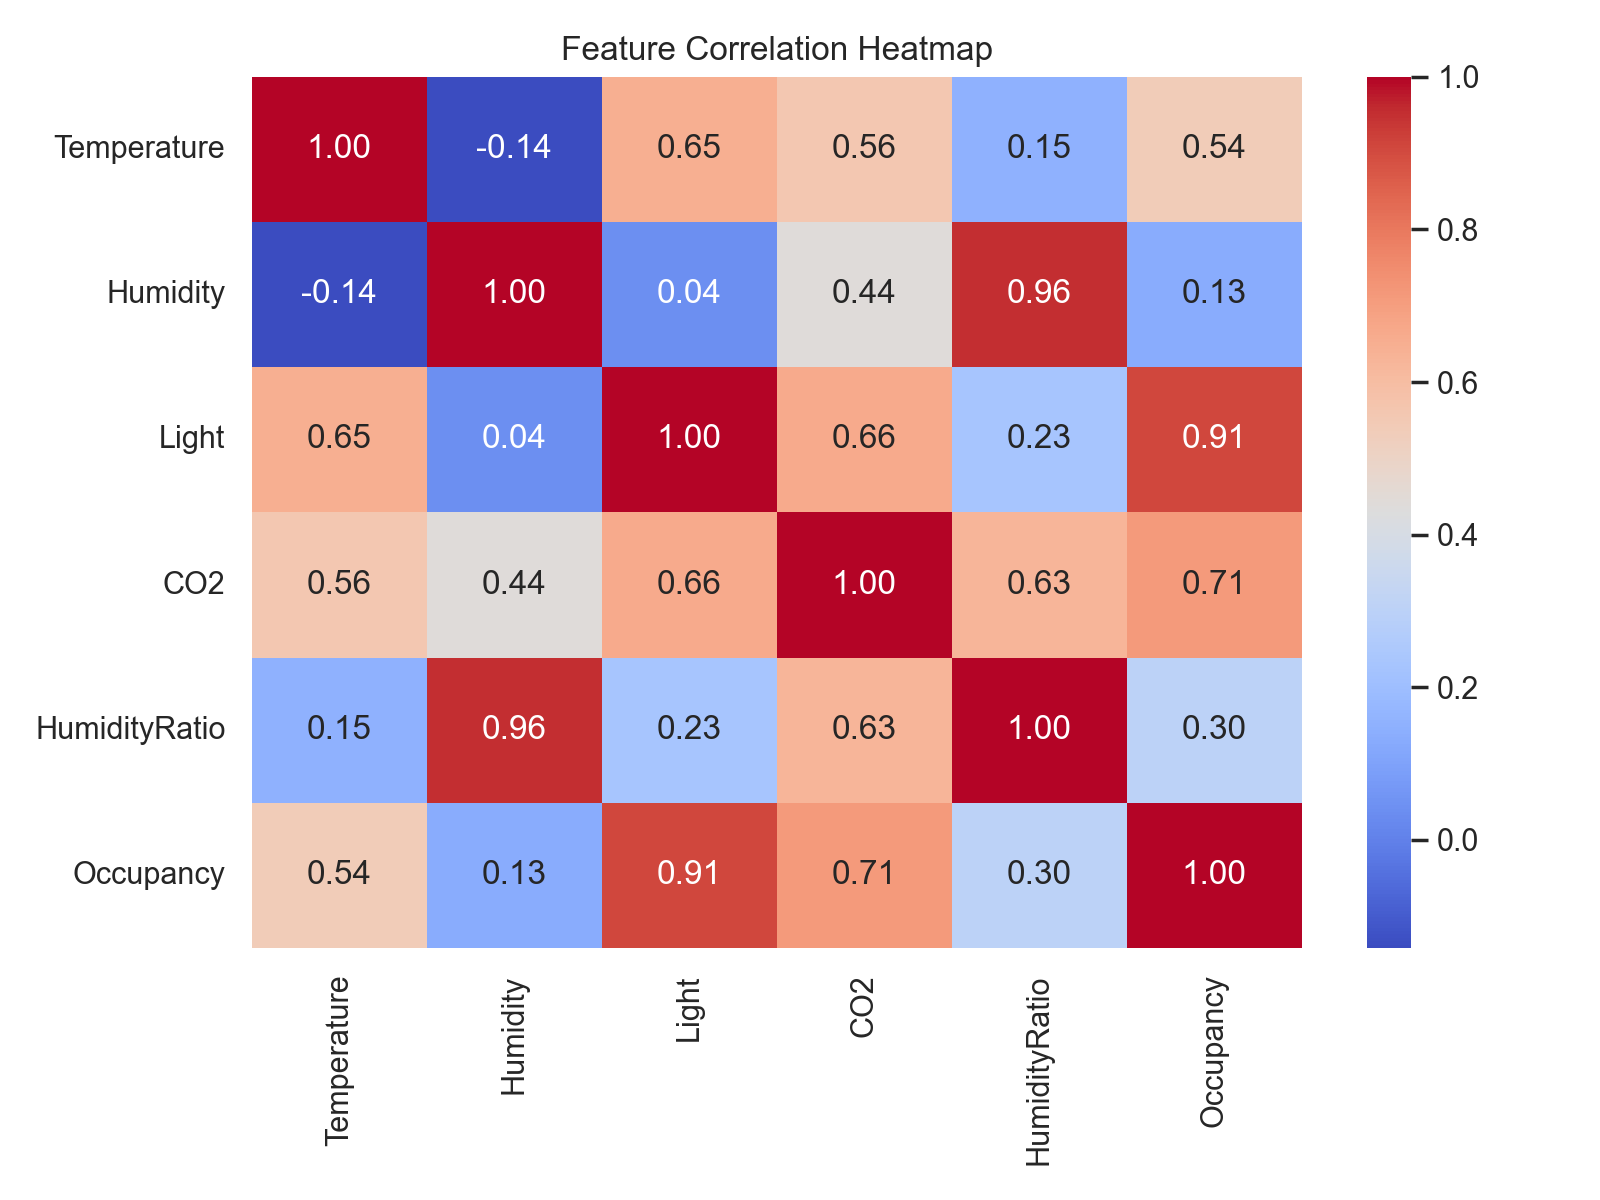
\includegraphics[width=0.9\textwidth]{figures/correlation_heatmap.png}
    \caption{Feature correlation heatmap. Light and CO$_2$ show the strongest relationship with occupancy.}
\end{figure}

\section{Results}
\subsection{Validation Results}
The validation results are shown in Table~\ref{tab:validationresults}.

\begin{table}[H]
\centering
\caption{Validation Results}
\label{tab:validationresults}
\begin{tabular}{lrrrr}
\toprule
Model & Accuracy & Precision & Recall & F1 \\
\midrule
Logistic Regression scaled & 0.9771 & 0.9470 & 0.9928 & 0.9694 \\
Logistic Regression unscaled & 0.9764 & 0.9469 & 0.9907 & 0.9683 \\
Random Forest & 0.9501 & 0.9458 & 0.9156 & 0.9305 \\
\bottomrule
\end{tabular}
\end{table}

The scaled Logistic Regression model was the best model on the validation split. Scaling only slightly improved the Logistic Regression result, but the improvement was consistent enough to justify using the scaled version for the final evaluation.

\subsection{Validation Confusion Matrices}
These matrices show that Logistic Regression produced far fewer false negatives than Random Forest on the validation split. That difference is reflected in the higher recall and F1 score for Logistic Regression.

\begin{figure}[H]
    \centering
    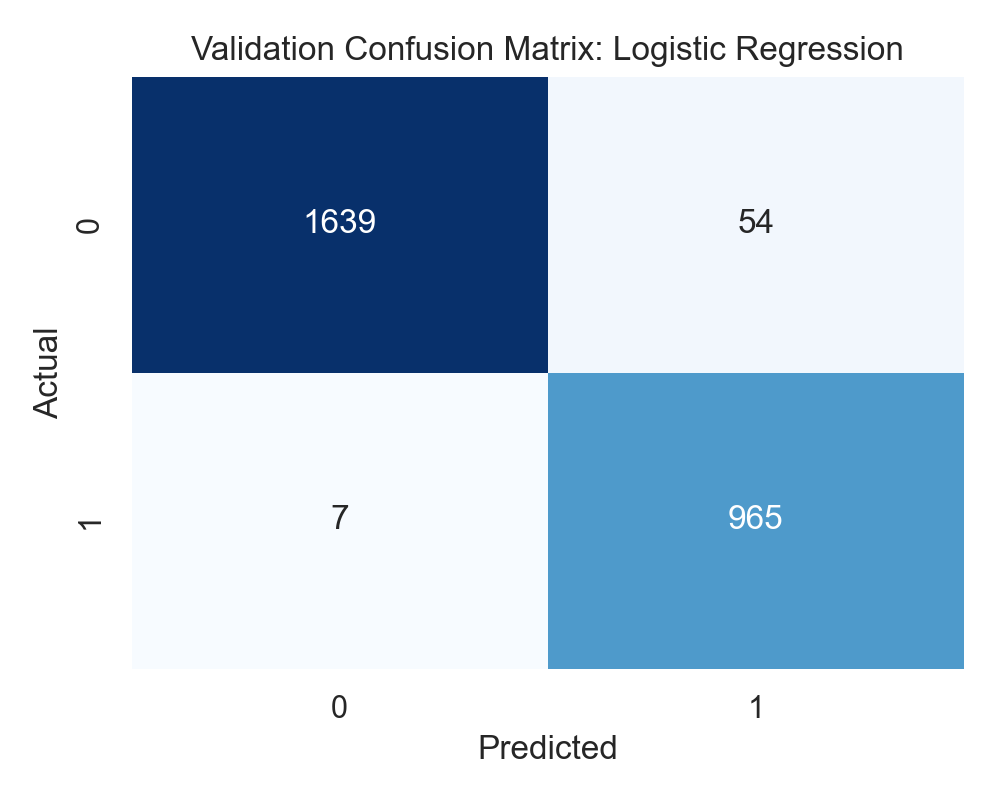
\includegraphics[width=0.47\textwidth]{figures/validation_confusion_logistic_regression.png}
    \hfill
    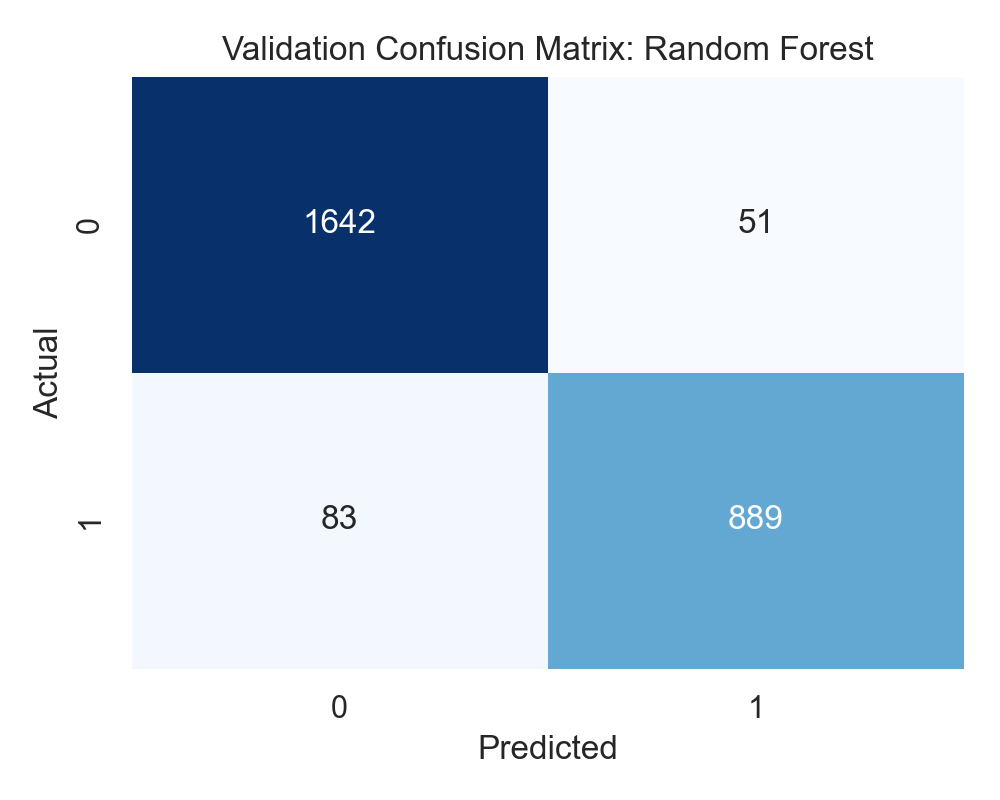
\includegraphics[width=0.47\textwidth]{figures/validation_confusion_random_forest.png}
    \caption{Validation confusion matrices for Logistic Regression and Random Forest.}
\end{figure}

\subsection{Final Holdout Test Results}
After model selection, the scaled Logistic Regression and Random Forest models were retrained on the combined training and validation data and evaluated on the final holdout split.

\begin{table}[H]
\centering
\caption{Holdout Test Results}
\begin{tabular}{lrrrr}
\toprule
Model & Accuracy & Precision & Recall & F1 \\
\midrule
Logistic Regression scaled & 0.9925 & 0.9718 & 0.9932 & 0.9824 \\
Random Forest & 0.9867 & 0.9436 & 0.9961 & 0.9691 \\
\bottomrule
\end{tabular}
\end{table}

The scaled Logistic Regression model again produced the best F1 score, confirming that the simpler model was sufficient for this dataset. Random Forest achieved slightly higher recall, but it did so at the cost of lower precision and lower overall F1 score.

\subsection{Holdout Test Confusion Matrices}
The Logistic Regression model made fewer total errors on the holdout set, especially fewer false positives than Random Forest.

\begin{figure}[H]
    \centering
    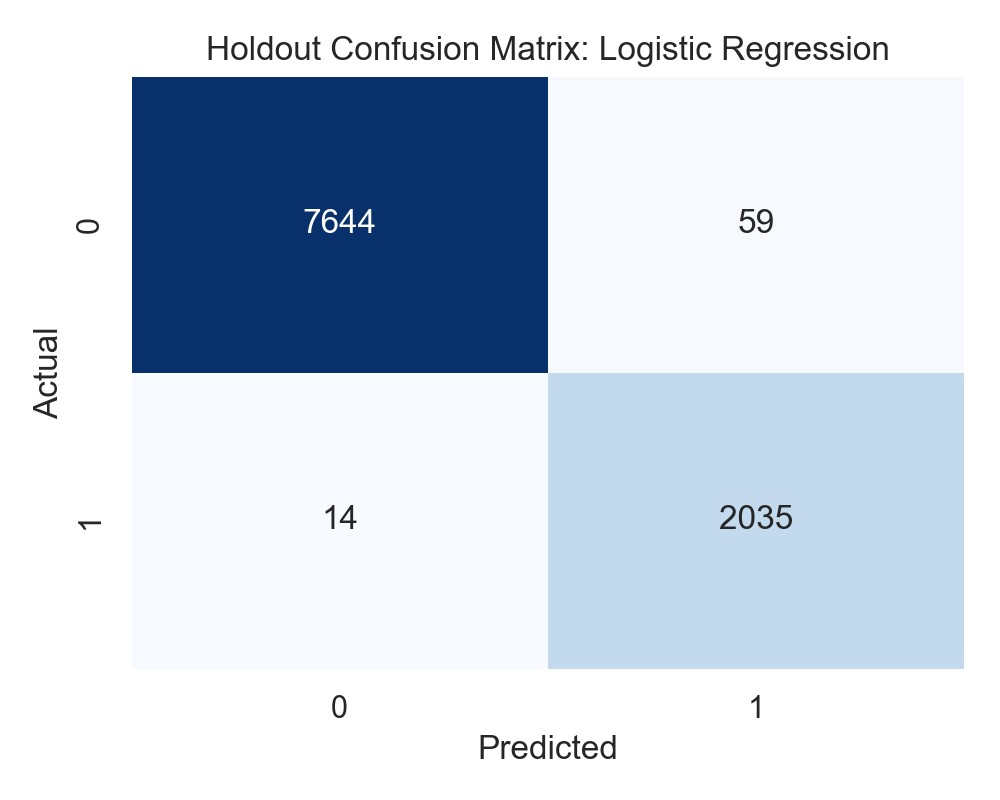
\includegraphics[width=0.47\textwidth]{figures/test_confusion_logistic_regression.png}
    \hfill
    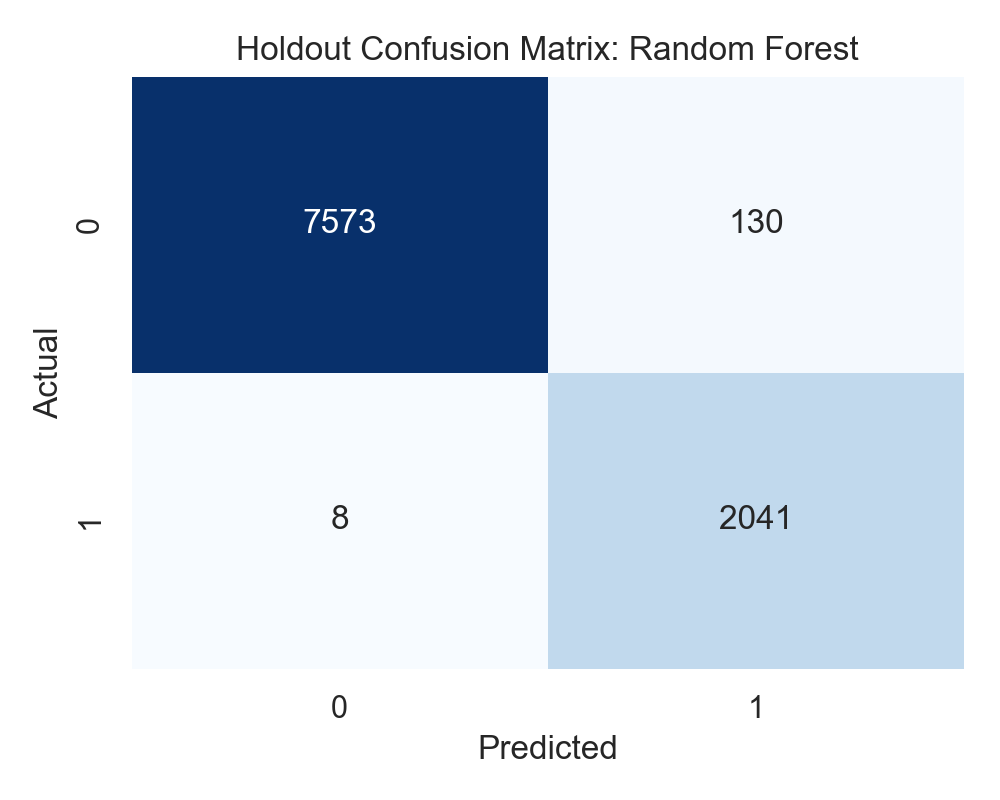
\includegraphics[width=0.47\textwidth]{figures/test_confusion_random_forest.png}
    \caption{Holdout test confusion matrices for Logistic Regression and Random Forest.}
\end{figure}

\section{Model Interpretation}
\subsection{Logistic Regression Coefficients}
The largest absolute Logistic Regression coefficients were Light, CO$_2$, Temperature, Humidity, and HumidityRatio, with Light having the strongest effect. This suggests that higher light levels and higher CO$_2$ values were strong indicators of occupancy in the fitted model.

\subsection{Random Forest Feature Importance}
The Random Forest feature importance values are shown in Figure~\ref{fig:rfimportance}.

\begin{table}[H]
\centering
\caption{Random Forest Feature Importance}
\begin{tabular}{lr}
\toprule
Feature & Importance \\
\midrule
Light & 0.6127 \\
CO$_2$ & 0.2272 \\
Temperature & 0.0962 \\
HumidityRatio & 0.0404 \\
Humidity & 0.0235 \\
\bottomrule
\end{tabular}
\end{table}

\begin{figure}[H]
    \centering
    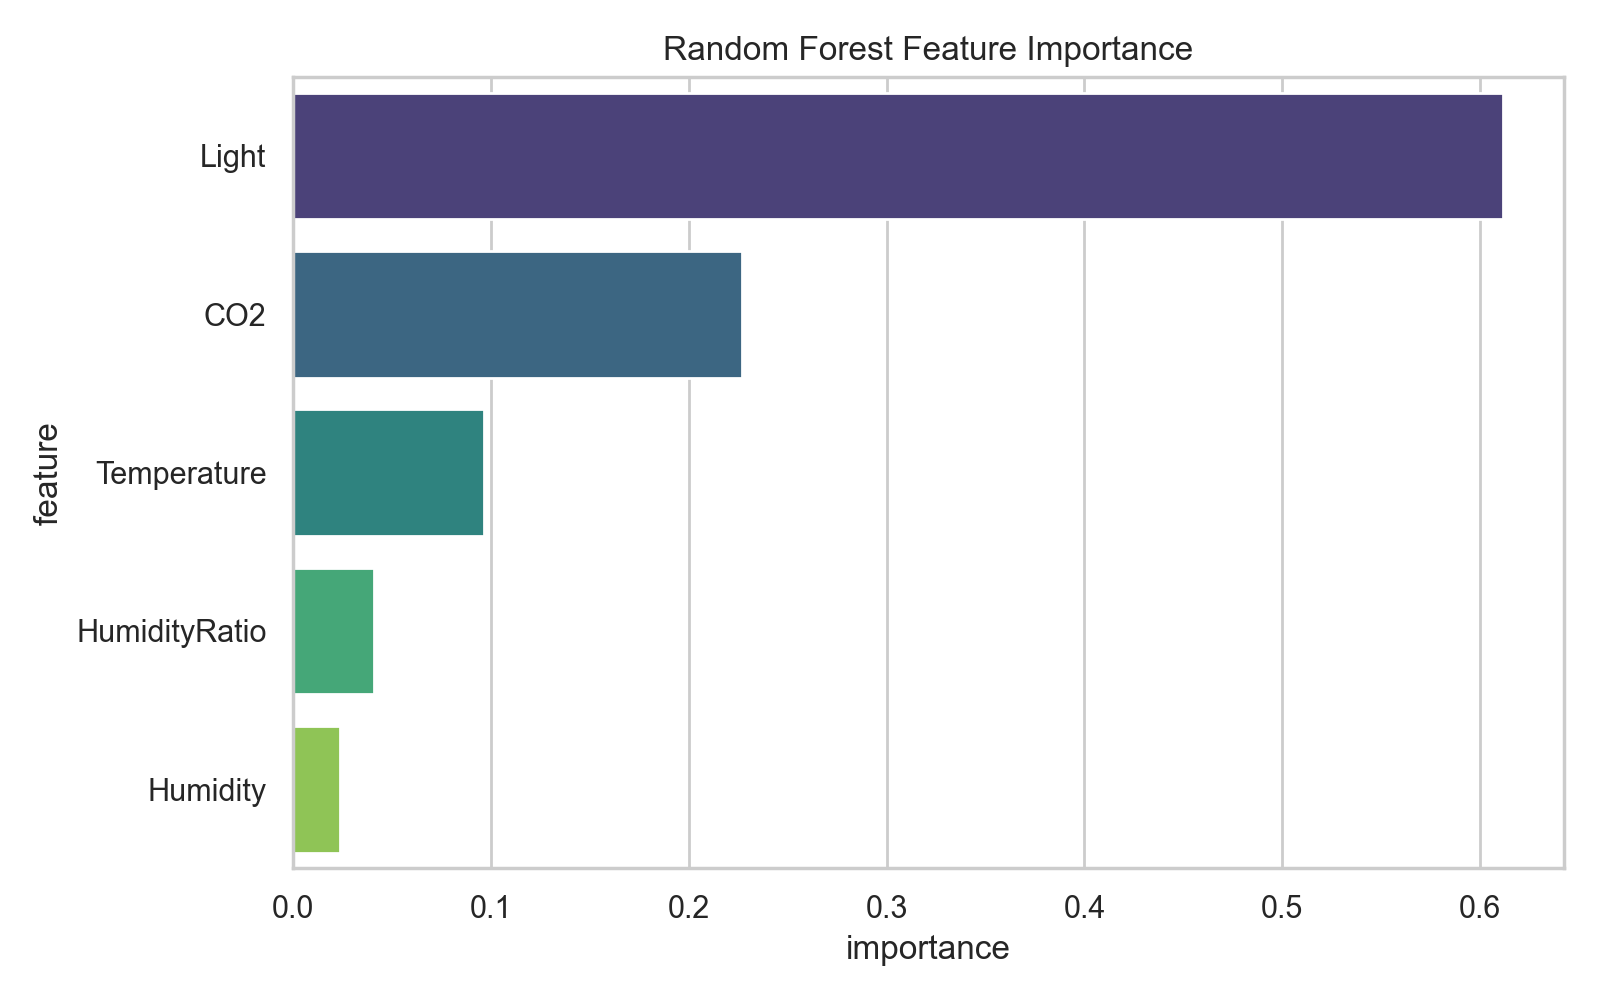
\includegraphics[width=0.85\textwidth]{figures/random_forest_feature_importance.png}
    \caption{Random Forest feature importance plot.}
    \label{fig:rfimportance}
\end{figure}

Both models indicate that Light and CO$_2$ are the most informative signals. This is a sensible result because these variables change noticeably when people are present in a room.

\section{Discussion}
The main goal of the project was to compare Logistic Regression and Random Forest on the room occupancy detection task. Based on the results, Logistic Regression performed better than Random Forest on both the validation and holdout splits. This is an important result because it shows that a relatively simple model can work extremely well on this dataset.

There are several possible reasons for this outcome. First, the relationship between occupancy and the sensor variables may be close to linearly separable once the data is scaled properly. Second, the strongest features, especially Light and CO$_2$, may already provide enough discriminative power that a more flexible model does not provide much additional benefit. Third, the Random Forest model may be more prone to small classification tradeoffs that increase recall but reduce precision.

Scaling had only a small effect on Logistic Regression, but the scaled version still outperformed the unscaled version on the validation split. That result supports the standard machine learning practice of scaling features before fitting linear models.

One limitation of this project is that the \texttt{date} field was not engineered into time based features such as hour of day or day of week. Adding those could potentially improve performance further. Another limitation is that the experiments focused on two standard algorithms rather than a wider benchmark set. Even so, the project successfully met its original scope and provided a clear comparison between a simple baseline and a more complex ensemble method.

\section{Conclusion}
This project demonstrated that room occupancy can be predicted accurately using environmental sensor data from a smart building setting. Logistic Regression and Random Forest were both effective, but Logistic Regression with feature scaling gave the best overall performance. The best holdout result was an F1 score of 0.9824, which shows that the sensor features are highly informative for occupancy detection.

The results also showed that Light and CO$_2$ were the most influential predictors across both models. Overall, the project supports the idea that non invasive sensors can be used to build accurate occupancy detection systems for practical IoT applications such as energy management and building automation.

\section{References}
\begin{enumerate}
    \item Candanedo, L. M., \& Feldheim, V. (2016). Accurate occupancy detection of an office room from light, temperature, humidity and CO$_2$ measurements using statistical learning models. \textit{Energy and Buildings, 112}, 28 to 39.
    \item UCI Machine Learning Repository. Occupancy Detection Data Set.
    \item Zhang, W., Han, K., Costa, G., \& Li, J. (2022). A review on occupancy prediction through machine learning for enhancing energy efficiency, air quality and thermal comfort in the built environment. \textit{Renewable and Sustainable Energy Reviews}.
\end{enumerate}

\end{document}
